\begin{frame}[label=gnss_ls_bk]
    \frametitle{GNSS: Developing a Least Squares Estimator}
    With 4+ bistatic range measurements, the meteor trail's reflection point can be estimated: 
    \begin{columns}
        \begin{column}{0.5\textwidth}
            {\setlength{\leftmargini}{1em} \begin{enumerate}
                \item Develop a \alert{ measurement model}, relating:  
                \begin{columns}
                    \begin{column}{0.5\linewidth }
                        {\setlength{\leftmargini}{3em} \begin{itemize} \scriptsize
                            \item[\(\blacktriangleright\)] \(\rho\): bistatic range
                            \item[\(\blacktriangleright\)] \(\mathbf{r}^{T}\): \textcolor{blue}{\textbf{TX}} location
                        \end{itemize}}
                    \end{column}
                    \begin{column}{0.5\linewidth}
                        \begin{itemize} \scriptsize
                            \item[\(\blacktriangleright\)] \(\mathbf{r}^R\): \textcolor{red}{\textbf{RX}} location
                            \item[\(\blacktriangleright\)] \(\mathbf{r}^s\): reflection point 
                        \end{itemize}
                    \end{column}
                \end{columns}                
            \end{enumerate}}
        \end{column}
        \begin{column}{0.5\textwidth}
            \scriptsize \begin{equation*} 
                \rho\left( \mathbf{r}^{s} \right) = \sqrt{\left( \mathbf{r}^{R}-\mathbf{r}^{s} \right)^{2}} + \sqrt{\left( \mathbf{r}^{T}-\mathbf{r}^{s} \right)^{2}} + \varepsilon
            \end{equation*}
        \end{column}
    \end{columns}
    %
    \begin{columns}
        \begin{column}{0.5\textwidth}
            {\setlength{\leftmargini}{1em} \begin{enumerate}   \setcounter{enumi}{1}
                \item \alert{Linearize the model} about some initial guess \(\mathbf{r}_0^s\)
            \end{enumerate}}
        \end{column}
        \begin{column}{0.5\textwidth}
            \scriptsize \begin{equation*}
                \rho \left( \mathbf{r}^{s} \right) \approx  \rho\left( \mathbf{r}^{s}_{0} \right) + \left. \frac{\partial \rho}{\partial \mathbf{r}^{s} } \right|_{\mathbf{r}^{s} = \mathbf{r}^{s}_0} \left( \mathbf{r}^{s} - \mathbf{r}^{s}_{0} \right)^{\top}
            \end{equation*}
        \end{column}
    \end{columns}
    %
    \begin{columns}
        \begin{column}{0.5\textwidth}
             {\setlength{\leftmargini}{1em} \begin{enumerate}   \setcounter{enumi}{2}
                \item \alert{Solve for the deviation} from the initial guess, \(\delta \mathbf{r} = \mathbf{r}^{s} - \mathbf{r}^{s}_{0}\)
            \end{enumerate}}
        \end{column}
        \begin{column}{0.5\textwidth}
            \scriptsize \begin{equation*}
                 \delta\rho =  \rho\left( \mathbf{r}^{s} \right)  -  \rho\left( \mathbf{r}^{s}_{0} \right) = \left. \frac{\partial \rho}{\partial \mathbf{r}^{s} } \right|_{\mathbf{r}^{s} = \mathbf{r}^{s}_0} \delta \mathbf{r}^{\top} + \varepsilon
            \end{equation*}
        \end{column}
    \end{columns}
    %
    \begin{columns}
        \begin{column}{0.5\textwidth}
            {\setlength{\leftmargini}{1em} \begin{enumerate}   \setcounter{enumi}{3}
                \item Put into \alert{least squares formulation} to find best position solution
            \end{enumerate}}
        \end{column}
        \begin{column}{0.5\textwidth}
            \scriptsize \begin{equation*}
                \delta\boldsymbol{\rho} = \mathbf{G}  \delta \mathbf{r}^{\top} + \boldsymbol{\varepsilon} \xrightarrow[]{}  \delta \hat{\mathbf{r}} = \left( \mathbf{G}^{\top} \mathbf{G} \right)^{-1} \mathbf{G}^{\top} \delta \boldsymbol{\rho}
            \end{equation*}
        \end{column}
    \end{columns}
    %
    \begin{columns}
        \begin{column}{0.5\textwidth}
            {\setlength{\leftmargini}{1em} \begin{enumerate}   \setcounter{enumi}{4}
                \item \alert{Update the initial guess}: set \(\mathbf{r}_0^s = \hat{\mathbf{r}}\)
            \end{enumerate}}
        \end{column}
        \begin{column}{0.5\textwidth}
            \scriptsize \begin{equation*}
                \hat{\mathbf{r}} = \mathbf{r}_0^s + \delta \hat{\mathbf{r}}
            \end{equation*}
        \end{column}
    \end{columns}
    %
    \begin{columns}
        \begin{column}{0.5\textwidth}
            {\setlength{\leftmargini}{1em} \begin{enumerate} \setcounter{enumi}{5}
                \item \alert{Repeat} until convergence
            \end{enumerate}}
        \end{column}
        \begin{column}{0.5\textwidth}
            
        \end{column}
    \end{columns}
\end{frame}

\begin{frame}[t, label=missed_weak]
    \frametitle{What Meteors are Missed?}
    \centering
    A: \alert{Weak reflection} towards \textcolor{red}{\textbf{RX}} \uncover<2->{\(\xrightarrow[]{}\) \alert{Increase \textcolor{blue}{\textbf{TX}} power}}

    \begin{tikzpicture}[remember picture, overlay]
        \node<1>[anchor=south east] (img) at ([xshift=-0.1cm, yshift=0.55cm]current page.south east) {
            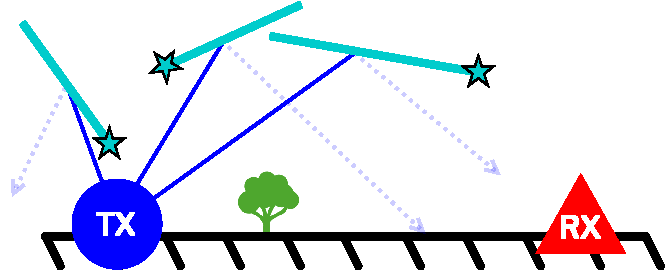
\includegraphics[height=6cm]{img/improve_link.pdf}%
        };
        \node<2->[anchor=south east] at ([xshift=-0.1cm, yshift=0.55cm]current page.south east) {
            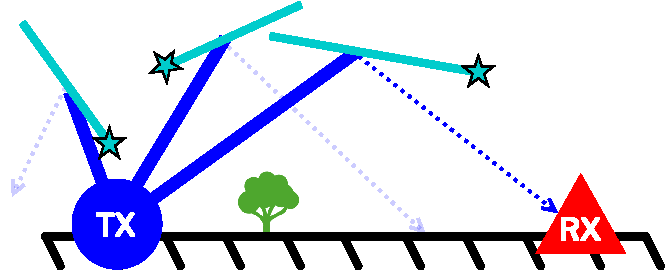
\includegraphics[height=6cm]{img/increase_power.pdf}%
        };
        \node[circle, draw=yellow, fill=yellow!30, thick, minimum size=4mm] at ([xshift=1.85cm, yshift=-1.5cm]img.north west) {C};
        \node[circle, draw=yellow, fill=yellow!30, thick, minimum size=4mm] at ([xshift=-2.25cm, yshift=-0.35cm]img.north) {B};
        \node[circle, draw=yellow, fill=yellow!30, thick, minimum size=4mm] at ([xshift=0.4cm, yshift=-0.6cm]img.north) {A};
    \end{tikzpicture}
\end{frame}

\begin{frame}[t, label=missed_away]
    \frametitle{What Meteors are Missed?}
    \centering
    B: Reflects power within network, \alert{away from \textcolor{red}{\textbf{RX}}} \uncover<2->{\(\xrightarrow[]{}\) \alert{Increase network density}}

    \begin{tikzpicture}[remember picture, overlay]
        \node<1>[anchor=south east] (img) at ([xshift=-0.1cm, yshift=0.55cm]current page.south east) {
            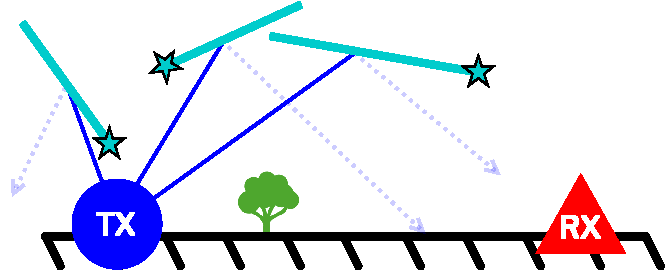
\includegraphics[height=6cm]{img/improve_link.pdf}%
        };
        \node<2->[anchor=south east] at ([xshift=-0.1cm, yshift=0.55cm]current page.south east) {
            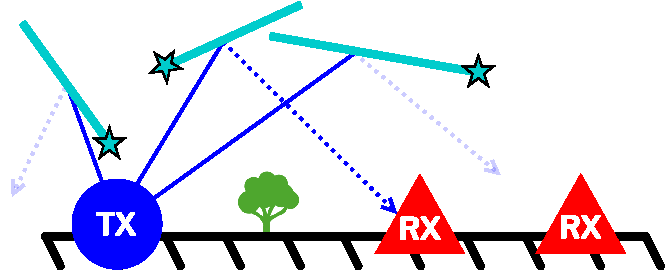
\includegraphics[height=6cm]{img/increase_density.pdf}%
        };
        \node[circle, draw=yellow, fill=yellow!30, thick, minimum size=4mm] at ([xshift=1.85cm, yshift=-1.5cm]img.north west) {C};
        \node[circle, draw=yellow, fill=yellow!30, thick, minimum size=4mm] at ([xshift=-2.25cm, yshift=-0.35cm]img.north) {B};
        \node[circle, draw=yellow, fill=yellow!30, thick, minimum size=4mm] at ([xshift=0.4cm, yshift=-0.6cm]img.north) {A};
    \end{tikzpicture}
\end{frame}

\begin{frame}[t, label=missed_outside]
    \frametitle{What Meteors are Missed?}
    \centering
    C: Reflects power \alert{outside network} \uncover<2->{\(\xrightarrow[]{}\) \alert{Increase network coverage}}

    \begin{tikzpicture}[remember picture, overlay]
        \node<1>[anchor=south east] (img) at ([xshift=-0.1cm, yshift=0.55cm]current page.south east) {
            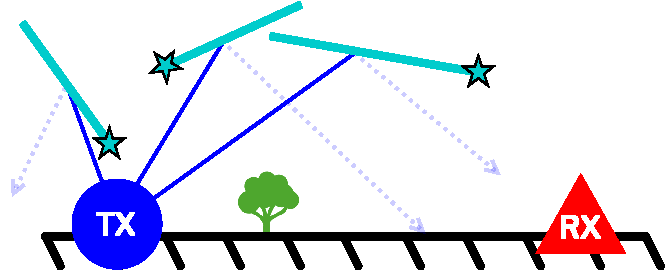
\includegraphics[height=6cm]{img/improve_link.pdf}%
        };
        \node<2->[anchor=south east] at ([xshift=-0.1cm, yshift=0.55cm]current page.south east) {
            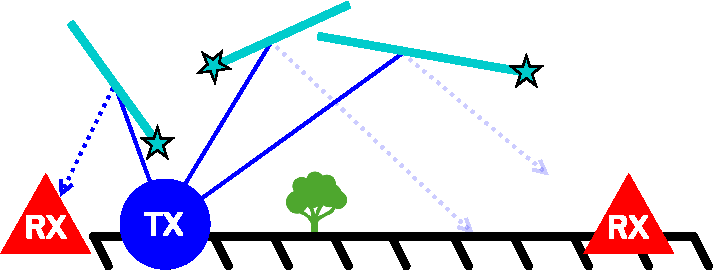
\includegraphics[height=6cm]{img/increase_coverage.pdf}%
        };
        \node[circle, draw=yellow, fill=yellow!30, thick, minimum size=4mm] at ([xshift=1.85cm, yshift=-1.5cm]img.north west) {C};
        \node[circle, draw=yellow, fill=yellow!30, thick, minimum size=4mm] at ([xshift=-2.25cm, yshift=-0.35cm]img.north) {B};
        \node[circle, draw=yellow, fill=yellow!30, thick, minimum size=4mm] at ([xshift=0.4cm, yshift=-0.6cm]img.north) {A};
    \end{tikzpicture}
\end{frame}